% compile with
%   pdflatex --shel-escape p02-variaveis
% or
%   latexmk -pvc -pdf -latexoption=--shell-escape p02-variaveis
%

\documentclass[11pt,fleqn]{practice}

\usepackage[american voltages]{circuitikz}
\usepackage{cancel}

\begin{document}

\tcbset{lowerbox=ignored}

\institution{UFOP\quad DECOM}
\course{Programação de Computadores I}
\subtitle{Aula prática 2}
\title{Variáveis, Atribuição, Entrada e Saída}
% \author{José Romildo Malaquias\thanks{\url{romildo@iceb.ufop.br}}}
\date{2014--2}
\maketitle

\begin{abstract}
  Nesta aula o aluno deverá desenvolver programas simples para resolver
  problemas de cálculo usando \textbf{variáveis} e o \textbf{comando de
    atribuição}, e os \textbf{comandos de entrada e saída} de dados para
  interação com o usuário.

  % Também será explorada a noção de vetores para desenhar gráficos de
  % funções.
\end{abstract}

\tableofcontents

\section{Variáveis}

\textbf{Variável} é um local de armazenamento de dados na memória do
computador. Podemos entendê-la como uma \emph{caixinha} onde são
colocados os dados processados em um programa.

\begin{center}
  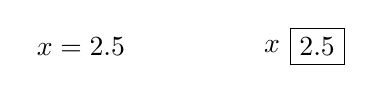
\begin{tikzpicture}
    \node[] (a) {$x = 2.5$};
    \node[draw,label=left:$x$,node distance=3cm,right of=a] {$2.5$};
  \end{tikzpicture}
\end{center}

Variáveis são identificadas por um \textbf{nome} que consiste em uma
sequência de letras, dígitos decimais, e caracteres especiais
(\texttt{\%}, \texttt{\_}, \texttt{\#}, \texttt{!}, \texttt{\$},
\texttt{?}), devendo começar com uma letra ou com o caracter
\texttt{\%}. Letras maíúsclas e minúsculas são consideradas
diferentes. Somente os 24 primeiros caracters do nome de uma variável
são significativos.

São nomes de variáveis válidos: \texttt{altura}, \texttt{peso1},
\texttt{quantidade\_tomates}, \texttt{numeroAlunos}, \texttt{\%pi}. Não
são nomes de variáveis válidos: \texttt{10anos}, \texttt{\_idade},
\texttt{media final}.

A operação de \textbf{atribuição} é utilizada para armazenar um valor em
uma variável. Sua forma básica é:
\begin{center}
  \emph{variável} = \emph{expressão}
\end{center}
Quando executado, este comando avalia a expressão e armazena o seu valor
na variável. O valor anteriormente armazenado na variável é perdido.

\begin{center}
  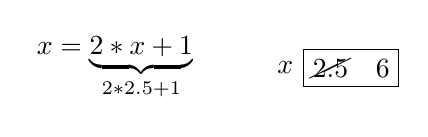
\begin{tikzpicture}
    \node[] (a) {$x = \underbrace{2*x + 1}_{2*2.5 + 1}$};
    \node[draw,label=left:$x$,node distance=3cm,right of=a] {\cancel{$2.5$}\quad $6$};
  \end{tikzpicture}
\end{center}

Para \textbf{acessar} o valor de uma variável basta usar o nome da
variável em uma expressão.


\section{Entrada de dados}

\begin{description}
  \item [\texttt{input(\textsl{mensagem})}]\mbox{}\newline Exibe
  \textsl{mensagem} (uma string ou cadeia de caracteres) na tela e
  espera uma entrada pelo teclado, e então retorna o valor numérico da
  expressão digitada pelo usuário.

  \item [\texttt{input(\textsl{mensagem}, "string")}]
  \item [\texttt{input(\textsl{mensagem}, "s")}]\mbox{}\newline Exibe
  \textsl{mensagem} (uma string ou cadeia de caracteres) na tela e
  espera uma entrada pelo teclado, e então retorna a linha digitada pelo
  usuário como uma string (cadeia de caracteres).
\end{description}

Exemplos:

\begin{lst}{text}
-->input("digite um número: ")
digite um número: 135
 ans  =
 
    135.  

-->input("digite o valor desejado: ")
digite o valor desejado: 2 + 3*4
 ans  =
 
    14.  
 
-->input("Nome do cliente: ", "string")
Nome do cliente: Manoel da Silva
 ans  =
 
 Manoel da Silva   

-->idade = input("idade do cliente: ")
idade do cliente: 17
 idade  =
 
    17.  
\end{lst}

\section{Saída de dados}

\begin{description}
  \item [\texttt{disp(\textsl{x$_1$}, \ldots, \textsl{x$_n$})}]\mbox{}\\
  Exibe os valores dos objetos \textsl{x$_1$}, \ldots, \textsl{x$_n$} na
  tela, em ordem inversa.

  \item [\texttt{printf(\textsl{formato}, \textsl{a$_1$}, \ldots, \textsl{a$_n$})}]\mbox{}\\
  Exibe na tela a string \textsl{formato}, inserindo os valores das expressões
  \textsl{a$_1$}, \ldots, \textsl{a$_n$} nas posições indicadas pelos
  formatadores presentes em \textsl{formato}.

  Alguns formatadores:
  \begin{center}
    \begin{tabular}{ll}\hline
      \textbf{formatador} & \textbf{formatação} \\\hline
      \texttt{\%s} & uma string (cadeia de caracteres) \\\hline
      \texttt{\%i} ou \texttt{\%d} & um número inteiro em notação decimal \\\hline
      \texttt{\%f} & um número real em notação decimal \\\hline
      \texttt{\%e} ou \texttt{\%E} & um número real em notação científica \\\hline
      \texttt{\%g} ou \texttt{\%G} & um número real no estilo de \texttt{f}, \texttt{e} ou \texttt{E}, o que for mais adequado \\\hline
      \texttt{\%\%} & insere um \texttt{\%} \\\hline
    \end{tabular}
  \end{center}

  Logo após o caracter \texttt{\%} de um formatador pode-se informar o
  tamanho mínimo do campo usado para inserir o valor. Por exemplo
  \texttt{\%12i} insere um número inteiro usando um espaço mínimo de 12
  caracteres.

  Nos formatadores de números fracionários pode-se informar o número de
  casas decimais logo após o tamanho do campo. Por exemplo
  \texttt{\%10.5f} insere um número fracionário usando um espaço mínimo
  de 10 caracteres (contando o ponto decimal), com 5 casas decimais.

  Um \texttt{-} antes do tamanho do campo alinha à esquerda. O padrão é
  alinhar à direita.
\end{description}

Strings podem conter \textbf{sequências de escape}, usuais na
represesntação de caracteres não gráficos:
\begin{description}
  \item [\texttt{\textbackslash n}] nova linha: quando exibido na tela
  faz com que o cursor avance para a próxima linha.
  \item [\texttt{\textbackslash t}] tabulação horizontal: quando exibido
  na tela faz com que o cursor avance para a próxima parada de
  tabulador. Normalmente existe uma parada de tabulador a cada 8 colunas
  na tela.
  \item [\texttt{\textbackslash \textbackslash}] o caracter
  \texttt{\textbackslash}.
\end{description}

Exemplos:
\begin{lst}{text}
-->printf('uma string: |%s|\n', 'Scilab');
uma string: |Scilab|
 
-->printf('um inteiro: |%d|\n', 10);
um inteiro: |10|
 
-->printf('um inteiro: |%4d|\n', 10);
um inteiro: |  10|
 
-->printf('um inteiro alinhado à esquerda: |%-4d|\n', 10);
um inteiro alinhado à esquerda: |10  |
 
-->printf('um float: |%d|\n', %pi);
um float: |3|
 
-->printf('um float em notação científica: |%3.2e|\n', %pi);
um float em notação científica: |3.14e+00|
 
-->printf('um float: |%3.2g|\n', %pi);
um float: |3.1|
\end{lst}

\section{Usando Scilab para resolver problemas}

\begin{task}[breakable]{Distância entre dois pontos no plano}{}
  A distância entre dois pontos $(x_1,y_1)$ e $(x_2,y_2)$ em um plano de
  coordenadas cartesianas é dada pela equação abaixo:
  \[ d = \sqrt{(x_1 - x_2)^2 + (y_1 - y_2)^2} \]
  Veja também a figura a seguir.

  \begin{center}
    \begin{tikzpicture}[domain=0:4]
      \draw[->] [very thin,color=gray] (-0.1,0) -- (4,0) node[anchor=north] {$x$};
      \draw[->] [very thin,color=gray] (0,-0.1) -- (0,4) node[anchor=east] {$y$};
      \draw[] (1,3) -- (3,1);
      \draw[dashed] (1,3) -- (1,1) -- (3,1);
      \draw[fill] (1,3) circle [radius=0.025] node[anchor=south] {$(x_1,y_1)$};
      \draw[fill] (3,1) circle [radius=0.025] node[anchor=north] {$(x_2,y_2)$};
    \end{tikzpicture}
    % \caption{Distância entre dois pontos em um plano cartesiano.}
    % \label{fig:dist}
  \end{center}

  Escreva um programa para calcular a distância entre dois pontos
  $(x1_,y_1)$ e $(x_2,y_2)$ especificados pelo usuário. Utilize boas
  práticas de programação em seu programa.

  Use o seu programa para calcular a distância entre os pontos $(-3,2)$
  e $(3,-6)$.

  \begin{runexample}
Cálculo da distância entre dois pontos
--------------------------------------
x1: -3
y1: 2
x2: 3
y2: -6

distância: 10
  \end{runexample}

  \tcblower
  \solution
  \lstinput{scilab}{listings/p02/distancia.sce}
\end{task}

\begin{task}[breakable]{Energia armazenada em uma mola}{}
  A força requerida para comprimir uma mola linear é dada pela equação
  \[ F = k x \] onde $F$ é a força em $N$ (newton), $x$ é a compressão
  da mola em $m$ (metro), e $k$ é a constante da mola em $N/m$.

  A energia potencial armazenada na mola comprimida é dada pela equação
  \[ E = \frac{1}{2} k x^2 \] onde $E$ é a energia em $J$ (joule).

  Escreva um programa para calcular a \emph{compressão} e a
  \emph{energia potencial} armazenada de uma mola, dadas a constante da
  mola e a força usada para comprimi-la.

  \begin{runexample}
Cálculo da energia armazenada em uma mola
-----------------------------------------
constante da mola (N/m): 250
força na mola (N): 30

compressão da mola: 0.120000 m
energia armazenada na mola: 1.800000 J
  \end{runexample}

  \tcblower
  \solution
  \lstinput{scilab}{listings/p02/mola.sce}
\end{task}

\begin{task}[breakable]{Receptor de rádio}{radio1}
  Uma versão simplificada da parte frontal de um receptor de rádio AM é
  apresentada na figura abaixo. Esse receptor é composto por um circuito
  que contém um resistor $R$, um capacitor $C$ e um indutor $L$
  conectados em série. O circuito é conectado a uma antena externa e
  aterrado conforme mostra a figura.

  \begin{center}
    \begin{circuitikz}[]
      \draw
        (0,0.8) node [ground] {} node [anchor=east] {Terra}
        to [short] (0,1)
        to [short] (6,1)
        to [R=$R$,v>=$V_R$] (6,4)
        to [C=$C$] (3,4)
        to [L=$L$] (1,4) node [antenna,xscale=-.7,] {} node [left=3em,above=2em,anchor=east] {Antena}
        (0,1) to [open,v>=$V_0$] (0,4)
        ;
    \end{circuitikz}
    % \caption{Distância entre dois pontos em um plano cartesiano.}
    % \label{fig:dist}
  \end{center}

  O circuito permite que o rádio selecione uma estação específica dentre
  as que transmitem na faixa AM. Na frequência de resonância do
  circuito, essencialmente todo o sinal $V_0$ da antena vai até o
  resistor, que representa o resto do rádio. Em outras palavras, o rádio
  recebe seu sinal mais forte na frequência de ressonância. A frequência
  de ressonância do circuito indutor-capacitor é dada pela equação
  \[ f_0 = \frac{1}{2 \pi \sqrt{L C}} \] onde $L$ é a indutância em $H$
  (henry) e $C$ é a capcitância em $F$ (farad).

  Escreva um programa que calcule a frequência de ressonância desse
  aparelho de rádio, dados valores específicos para $L$ e $C$ (o usuário
  do programa informa estes dados).

  Teste seu programa pelo cálculo da frequência do rádio quando $L=0,25
  mH$ e $C=0,10 nF$.
  \begin{runexample}
Cálculo da frequência de ressonância
------------------------------------
digite a indutância em henry: 0.25/1000
digite a capacitância em farad: 0.10/10^9

frequência de ressonância: 1.00658e+06 Hz
  \end{runexample}

  \tcblower
  \solution
  \lstinput{scilab}{listings/p02/ressonancia.sce}
\end{task}


% \section{Desenho de gráficos}

% Para desenhar um gráfico de uma maneira simples, siga os passos seguintes:
% \begin{enumerate}
%   \item É bom limpar a janela de gráficos (também chamada janela de
%   figuras) antes de começar a construir um novo desenho. Para tanto use
%   o comando \texttt{clf}.

%   \item Defina um vetor\footnote{Vetores são matrizes
%     unidimensionais. Um vetor linha é uma matriz contendo somente uma
%     linha. Um vetor coluna é uma matriz contendo somente uma coluna}
%   contendo as abscissas dos pontos a serem plotados. A notação de
%   progressão aritmética pode ser usada, indicando o limite inferior, a
%   razão, e o limite superior.

%   Exemplo:
%   \begin{lst}{scilab}
% // vetor linha formado pelos valores das
% // abscissas dos pontos a serem plotados

% // limite inferior: -pi
% // razão (ou passo): 0.2
% // limite superior: pi

% x = [-%pi : 0.2 : %pi];
%   \end{lst}

%   \item Defina outro vetor linha contendo as ordenadas dos pontos a
%   serem plotados. Pode-se usar operações aritméticas ou funções com
%   vetores para construir este vetor a partir do vetor das abscissas.

%   Para realizar uma operação entre um escalar $k$ e cada elemento de uma
%   matriz $A$, produzindo a matriz dos resultados, temos:
%   \begin{center}
%     \begin{tabular}{p{2cm}l} \hline
%       \textbf{operação} & \textbf{descrição} \\\hline
%       \texttt{$k$ + $A$}\newline \texttt{$A$ + $k$}  & adição \\\hline
%       \texttt{$k$ - $A$}\newline \texttt{$A$ - $k$}  & subtração \\\hline
%       \texttt{$k$ * $A$}\newline \texttt{$A$ * $k$}  & multiplicação \\\hline
%       \texttt{$A$ / $k$}\newline \texttt{$k$ ./ $A$}  & divisão \\\hline
%       \texttt{$A$ .\textasciicircum\ $k$}  & potenciação \\\hline
%     \end{tabular}
%   \end{center}

%   Para realizar uma operação com duas matrizes $A$ e $B$ entre os
%   elementos correspondentes, produzindo a matriz dos resultados, temos:
%   \begin{center}
%     \begin{tabular}{ll} \hline
%       \textbf{operação} & \textbf{descrição} \\\hline
%       \texttt{$A$ + $B$} & adição \\\hline
%       \texttt{$A$ - $B$} & subtração \\\hline
%       \texttt{$A$ .* $B$} & multiplicação \\\hline
%       \texttt{$A$ ./ $B$} & divisão \\\hline
%       \texttt{$A$ .\textasciicircum\ $B$} & potenciação \\\hline
%     \end{tabular}
%   \end{center}

%   Várias funções podem ser aplicadas a matrizes, e a função será
%   realizada individualmente com cada elemento da matriz, produzindo a
%   matriz dos resultados.

%   Exemplo:
%   \begin{lst}{scilab}
% // vetor linha formado pela aplicação da função
% // f(x) = x * sin(x) - x^3 / (2*pi)
% // a cada elemento do vetor das abscissas

% y = x .* sin(x) - x .^ 3 / (2*%pi);
%   \end{lst}

%   \item Para desenhar o gráfico, use a função \texttt{plot}, passando o
%   vetor das abscissas e o vetor das ordenadas como argumentos. Pode-se
%   desenhar vários gráficos ao mesmo tempo. Para cada gráfico use dois
%   vetores (abscissas e ordenadas).

%   A função \texttt{title} permite dar um título ao desenho.

%   As funções \texttt{xlabel} e \texttt{ylabel} podem ser usadas para
%   rotular os eixos do desenho.

%   A função \texttt{legend} coloca legendas nos gráficos desenhados.

%   A expressão \texttt{set(gca(), "grid", [1 1])} desenha uma grade.

%   Exemplo:
%   \begin{lst}{scilab}
% // desenha o gráfico
% plot(x, y);
% title("Gráfico de funções");
% xlabel("x");
% ylabel("y");
% legend("Resultado");
% set(gca(), "grid", [1 1]);
%   \end{lst}
%   A seguir temos o desenho produzido por este exemplo.
%   \begin{center}
%     \includegraphics[width=\linewidth]{images/grafico}
%   \end{center}
% \end{enumerate}

% \begin{task}{Posição e velocidade de uma bola \numex{2.10}}{}
%   Se uma bola estacionária é lançada da altura $h_0$ acima da superfície
%   da Terra, com velocidade vertical $v_0$, a posição e a velocidade da
%   bola como função do tempo serão dadas pelas equações
%   \[ h(t) = \frac{1}{2}gt^2 + v_0t + h_0 \]
%   \[ v(t) = gt + v_0 \] onde $g$ é a aceleração da gravidade
%   ($-9,8m/s^2$), $h$ é a altura acima da superfície da Terra (assumindo
%   ausência de atrito do ar) e $v$ é a componente vertical da velocidade.

%   Escreva um programa que solicite ao usuário a altura inicial da bola
%   em $m$ e a velocidade de lançamento da bola em $m/s$, depois desenhe a
%   altura e velocidade em função do tempo. Não deixe de incluir as
%   legendas apropriadas no seu desenho.

%   \begin{runexample}
% Lançamento de uma bola
% ----------------------
% altura inicial da bola (m): 20
% velociade de lançamento da bola (m/s): 46
%   \end{runexample}
%   \begin{center}
%     \includegraphics[width=\linewidth]{images/bola}
%   \end{center}

  % \tcblower
  % \solution
  % \lstinput{scilab}{listings/p03/bola.sce}
  % \includegraphics{listings/p03/bola.png}
% \end{task}

\end{document}
